\documentclass{article}

\usepackage{xeCJK}
\usepackage{fancyhdr}
\usepackage{extramarks}
\usepackage{amsmath}
\usepackage{amsthm}
\usepackage{amsfonts}
\usepackage{tikz}
\usepackage[plain]{algorithm}
\usepackage{algpseudocode}
\usepackage{enumerate}
\usepackage{xcolor, minted}
\usepackage[inline]{enumitem}
\usepackage{booktabs}
\usepackage{makecell}
\usepackage{multirow}
\usemintedstyle{colorful}
\definecolor{bg}{rgb}{0.95, 0.95, 0.95}
\definecolor{lk}{rgb}{0.5, 0.1, 0.1}
\setminted{bgcolor=bg,
           numbers=right,
           samepage}
\setmonofont{Droid Sans Mono for Powerline}

\usetikzlibrary{automata,positioning}

\usepackage[
  colorlinks,
  urlcolor=lk,
  linkcolor=black,
  citecolor=red,
  ]{hyperref}

\usepackage{tocloft}
\renewcommand\cfttoctitlefont{\huge\bfseries}
\renewcommand\cftsecfont{\Large\bfseries}
\renewcommand\cftsubsecfont{\large}
\renewcommand\cftsubsubsecfont{\large}
\setlength\cftbeforesecskip{20pt}
\setlength\cftbeforesubsecskip{10pt}
\setlength\cftbeforesubsubsecskip{8pt}

\setlength\parskip{0.8em}
\setlength\lineskip{0.5em}


%
% Basic Document Settings
%
\setmainfont[ItalicFont=Times New Roman Italic]{Arial}
\setCJKmainfont[ItalicFont=STKaiti, BoldFont=STHeiti]{STXihei}

\topmargin=-0.45in
\evensidemargin=0in
\oddsidemargin=0in
\textwidth=6.5in
\textheight=9.0in
\headsep=0.25in

\linespread{1.1}

\pagestyle{fancy}
\lhead{\reportAuthorName}
\chead{\reportMainTitle}
\rhead{\leftmark}
\cfoot{\thepage}

\renewcommand\headrulewidth{0.4pt}
\renewcommand\footrulewidth{0.4pt}

\setlength\parindent{0pt}

%
% Create Problem Sections
%


%
% Homework Details
%   - Title
%   - Due date
%   - Class
%   - Section/Time
%   - Instructor
%   - Author
%

\newcommand{\reportMainTitle}{Implementation of Branch Decision}
\newcommand{\reportTitle}{Lab\ \#4}
\newcommand{\reportDueTime}{May 31, 2020 at 23:59pm}
\newcommand{\reportClass}{Computer Architecture}
\newcommand{\reportClassTime}{}
\newcommand{\reportClassInstructor}{周学海}
\newcommand{\reportAuthorName}{魏剑宇}
\newcommand{\reportStudentNo}{PB17111586}

%
% Title Page
%

\title{
  \vspace{2in}
  \textbf{\reportMainTitle}\\
  \vspace{0.2in}
  \Large\textit{\reportClass:\ \reportTitle}\\
  \vspace{0.1in}
  \normalsize\vspace{0.1in}\small{Due\ on\ \reportDueTime}\\
  \vspace{3in}
}

\author{\reportAuthorName \\ \reportStudentNo}
\date{May 31, 2020}


%
% Various Helper Commands
%

% Useful for algorithms
\newcommand{\alg}[1]{\textsc{\bfseries \footnotesize #1}}

% For derivatives
\newcommand{\deriv}[1]{\frac{\mathrm{d}}{\mathrm{d}x} (#1)}

% For partial derivatives
\newcommand{\pderiv}[2]{\frac{\partial}{\partial #1} (#2)}

% Integral dx
\newcommand{\dx}{\mathrm{d}x}

% Alias for the Solution section header

% Probability commands: Expectation, Variance, Covariance, Bias
\newcommand{\E}{\mathrm{E}}
\newcommand{\Var}{\mathrm{Var}}
\newcommand{\Cov}{\mathrm{Cov}}
\newcommand{\Bias}{\mathrm{Bias}}

\begin{document}

\maketitle

\pagebreak

\tableofcontents\label{toc}

\pagebreak

\newpage

\section{实验环境和工具}
\begin{itemize}
  \item
    \textbf{Host OS}: macOS Mojave 10.14.6
  \item
    \textbf{Guest OS}: Ubuntu Bionic Beaver
  \item
    \textbf{VSCode}: 1.44.2
  \item
    \textbf{Vivado}: HL WebPack Edition
  \item
    \textbf{Git}: 2.20.1 (Apple Git-117)
\end{itemize}
本次实验 Simulation 部分在 Ubuntu 虚拟机中完成 (Vivado 没有提供 macOS 版本),代码编写在 mac 上使用 VSCode 完成.

我的做法是在虚拟机 vivado 创建项目时,将源码的文件夹添加进去的时候,不拷贝,而是映射到项目中。然后在 mac 上通过共享文件夹将源码映射到 ubuntu 上,这样,源码编辑和 Git 版本控制都可以在 mac 上完成,只需在仿真的时候切换到 Ubuntu。整个一套 workflow 还是非常流畅舒适的。

\section{Branch History Table}
下表中 target 表示既不在 BTB 中,也不是 PC\_IF+4,而是指令中决定的跳转地址。
\begin{table}[H]
  \centering
  \begin{tabular}{c c c c c c c}
    \toprule
    BTB & BHT & REAL & NPC\_PRED & flush & NPC\_REAL & BTB update \\
    \midrule
    Y   & Y   & Y    & BUF       & N     & BUF       & N          \\
    Y   & Y   & N    & BUF       & Y     & PC\_IF+4  & N          \\
    Y   & N   & Y    & PC\_IF+4  & Y     & BUF       & N          \\
    Y   & N   & N    & PC\_IF+4  & N     & PC\_IF+4  & N          \\
    N   & Y   & Y    & PC\_IF+4  & Y     & target    & Y          \\
    N   & Y   & N    & PC\_IF+4  & N     & PC\_IF+4  & N          \\
    N   & N   & Y    & PC\_IF+4  & Y     & target    & Y          \\
    N   & N   & N    & PC\_IF+4  & N     & PC\_IF+4  & N          \\
    \bottomrule
  \end{tabular}
  \caption{BHT 策略矩阵}
\end{table}

\section{性能测试 \& 分析}
下面在进行性能测试的时候,我都是截止到最后死循环的时候(而不是死循环前的那个遍历数组的循环).

例如,如下是矩阵乘法时结束的时间点:
\begin{figure}[H]
  \centering
  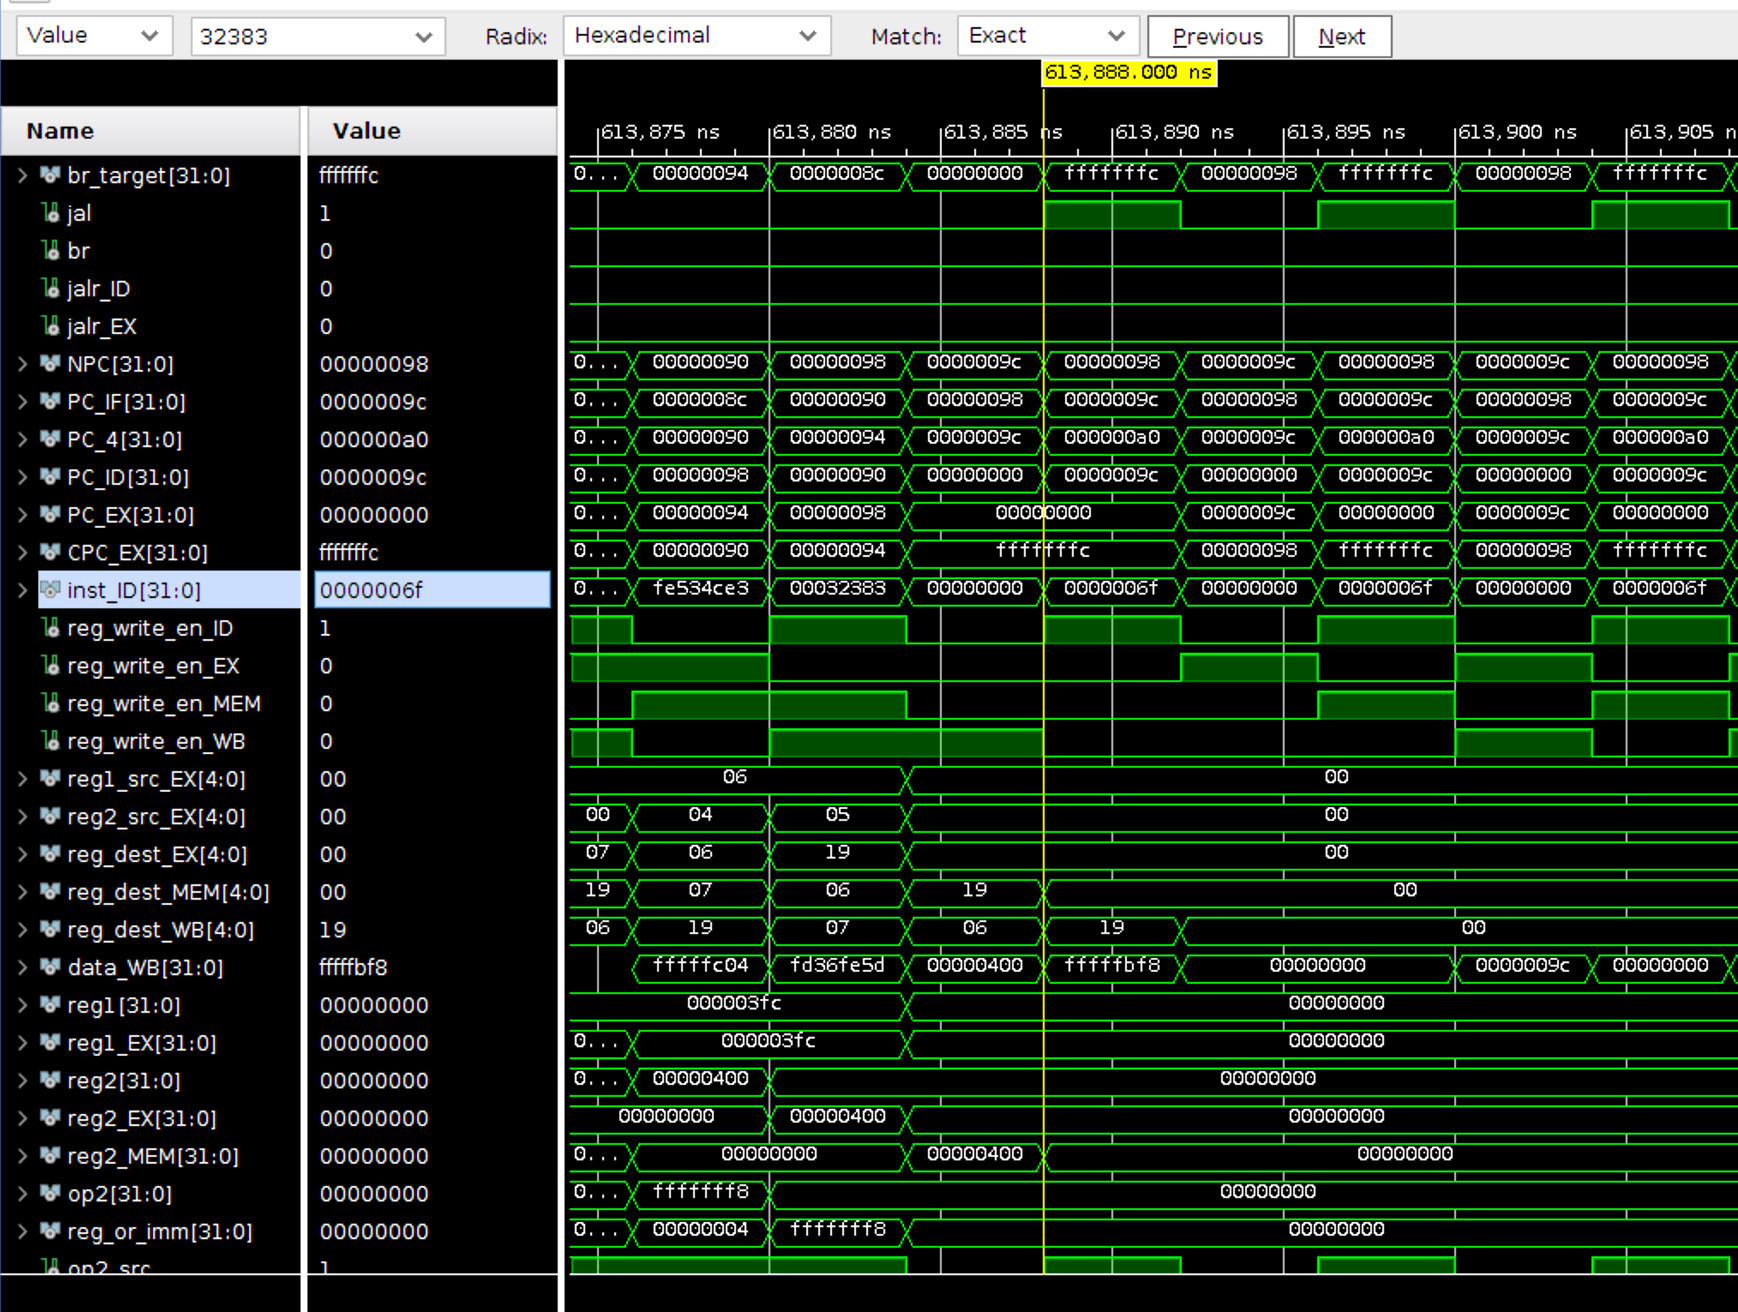
\includegraphics[width=10cm]{simulation.png}
\end{figure}

另外,对于 bht.S 和 btb.S 两个程序,由于最后没有死循环,直接截止到最后一个循环执行的时间即可.(之后指令是 XXX)

在测试的时候需要注意,其它几个程序都没问题,但对于 quicksort 需要保证内存是同一次生成的。因为内存是随机生成的,对其它的程序的运行流程没有影响,但对于排序会造成影响。

同时在测试的时候,我的 cache 使用的同一个参数 (WAY\_CNT=4, SET\_ADDR\_LEN=3, LINE\_ADDR\_LEN=3).

得到结果如下(矩阵乘法和排序皆使用默认参数):
\begin{table}[H]
  \centering
  \begin{tabular}{c c c c c c c c}
    \toprule
    程序名 & 分支策略 & 时间 (ns) & 加速比 & 正确次数 & 错误次数 & 总次数 & 正确率\\
    \midrule
    \multirow{3}{*}{matmul.s} & BHT & 613880 & 1.053 & 4342 & 282 & 4624 & 93.9\% \\
                              & BTB & 616016 & 1.049 & 4076 & 548 & 4624 & 88.1\% \\
                              & baseline & 646432 & 1 & 274 & 4350 & 4624 & 5.9\% \\
    \midrule
    \multirow{3}{*}{quicksort.s} & BHT & 159484 & 1.020 & 10475 & 1908 & 12383 & 84.6\% \\
                                 & BTB & 161692 & 1.006 & 8749 & 3634 & 12383 & 70.7\% \\
                                 & baseline & 162710 & 1 & 7871 & 4512 & 12383 & 63.6\% \\
    \midrule
    \multirow{3}{*}{btb.s} & BHT & 1260 & 1.616 & 98 & 3 & 101 & 97.0\% \\
                           & BTB & 1252 & 1.626 & 99 & 2 & 101 & 98.0\% \\
                           & baseline & 2036 & 1 & 1 & 100 & 101 & 1.0\% \\
    \midrule
    \multirow{3}{*}{bht.s} & BHT & 1472 & 1.454 & 95 & 15 & 120 & 79.2\% \\
                           & BTB & 1524 & 1.404 & 88 & 22 & 120 & 73.3\% \\
                           & baseline & 2140 & 1 & 11 & 99 & 120 & 9.2\% \\
    \bottomrule
  \end{tabular}
  \caption{性能测试}
  \label{tb:perf}
\end{table}
在上表 \ref{tb:perf} 中,baseline 代表“没有分支预测的情况”。但实际上,由于在我前面的实现中,我实现了静态的分支预测(永远预测不跳转),所以 baseline 代表的是一直预测不跳转的性能(也因此有预测正确的个数和不正确的个数).
\subsection{分支收益和分支代价}

分析实验数据,btb.s 这一行 BHT 和 BTB 的对比能够很清晰地展现出预测所带来的收益。对于 BHT 和 BTB 两种实现策略,预测正确的次数差了 1,而时间差了 8ns。每一个时钟周期是 4ns,这刚好是两个时钟周期的时间。也就是说,预测错误的分支代价是 2.

理论上进行分析,每次错误的预测,都会使得实际到 EX 段才会得出正确的分支结果,这样我们需要 flush 调已经取入的错误指令(也就是下一个周期的 ID 和 EX),这样,我们会浪费掉两个流水线周期,和实验的结果相符。

总体的分支收益上,我们可以观察实验数据,两种预测策略在不同程序上都得到了一定加速比,且正确率也不错。因此而带来的分支收益是 $正确率 \times 总次数 \times 8ns$.

\subsection{分支策略:BHT vs BTB}
我们可以发现,在快速排序和矩阵乘法中,BHT 都稍微优于 BTB. 只有在 btb.s 中 BTB 稍微更胜一筹。我们可以对比 btb.s 和 bht.s 这两个相对比较简单的程序,更容易分析一些。

观察这两个程序我们发现,bht.s 是一个双层循环,btb.s 是一个单层循环。在双层循环中,每一个内层循环的末尾都将是一个实际不跳转,内层循环的开头都将是一个实际跳转。如果使用 BTB 作为分支策略,那么每一次内层循环的末尾都将预测失败,且由于上一次内层循环的末尾预测跳转而实际不跳转,下一次开头时就会预测不跳转,但实际跳转。对于 bht 则没有这种情况。

分析实验结果 bht.s 中的 BHT 和 BTB,两者预测正确次数差了 7。在对应的程序中,内层循环执行了 10 次,除去第一次的内层和外层循环,BHT 会由于从 $00 \rightarrow 01 \rightarrow 11$ 需要两次跳转会多带来两次预测失败外,第 2-10 个内层循环的开始相比 BTB 会多预测正确 9 次。因此理论上分析确实应该相差 $9 - 2 = 7$ 次。

而对于 btb.s 这一个单层循环的程序,BHT 开头会多预测失败一次,所以刚好差 1。

\subsection{程序特点带来的不同收益:MatMul vs QuickSort}

对于这两个程序,我们可以发现动态分支预测相比静态预测的优势在矩阵乘法上体现的更明显。这一点是由程序的特点体现的。

矩阵乘法是一个三层循环,对于一个 16x16 的矩阵乘法,每一循环的宽度都是 16。这 16 个中,基本都会预测跳转并且实际也是跳转,也就是说分支的局部性很好。相邻的两次分支结果基本都是相同的,因此正确率预测吕也很高。而静态预测不跳转的 baseline 因此正确率也低了很多。

而对于 quicksort,在决定是否需要交换时,都需要考察具体的数据。也就是说,分支的结果受到了随机生成的数据的影响,几乎是没有规律的,分支预测的正确率也就低了很多。我们可以观察到,哪怕每次都直接预测不跳转,也能有 63.6\% 的正确率。

\section{代码设计}

下面我讲一下我是如何实现 BHT 的。因为也涵盖了 BTB,我就不单独介绍了。

\subsection{BTB \& BHT}

在实现中,我按照 README 中的说法,将 BTB 表设计成一个直接相连的 cache,是一种最朴素的实现。上一次已经实现了 cache 了,这一次也就驾轻就熟。
\begin{minted}{verilog}
wire [              2-1:0]   rd_word_addr;
wire [   SET_ADDR_LEN-1:0]    rd_set_addr;
wire [   TAG_ADDR_LEN-1:0]    rd_tag_addr;
wire [UNUSED_ADDR_LEN-1:0] rd_unused_addr;

wire [              2-1:0]   wr_word_addr;
wire [   SET_ADDR_LEN-1:0]    wr_set_addr;
wire [   TAG_ADDR_LEN-1:0]    wr_tag_addr;
wire [UNUSED_ADDR_LEN-1:0] wr_unused_addr;
\end{minted}
和上次一样,声明这样一些地址。要准备两份,一份是在流水线的 IF 段需要查询某个 BTB 表,一个是在 EX 段对应的结果得出后可能需要更新 BTB 表。这个 BTB 表的更新操作也和 cache 类似,所以就不在这里详述了。

BHT 表我索性直接设成和 BTB 一样大(都是 4096),主要是因为代码空间比较小所以资源够用。BHT 表的更新通过 case 来实现。
\begin{minted}{verilog}
if (taken) begin
  case (bht[wr_set_addr])
      2'b00: bht[wr_set_addr] <= 2'b01;
      2'b01: bht[wr_set_addr] <= 2'b11;
      2'b10: bht[wr_set_addr] <= 2'b11;
      2'b11: bht[wr_set_addr] <= 2'b11;
  endcase
end else begin
  case (bht[wr_set_addr])
      2'b00: bht[wr_set_addr] <= 2'b00;
      2'b01: bht[wr_set_addr] <= 2'b00;
      2'b10: bht[wr_set_addr] <= 2'b00;
      2'b11: bht[wr_set_addr] <= 2'b10;
  endcase
end
\end{minted}

最后,预测是否进行跳转就比较简单了:
\begin{minted}{verilog}
assign pred_take = valid[rd_set_addr] & (rd_tag_addr == buffer_tags[rd_set_addr]) & bht[rd_set_addr][1];
\end{minted}
也就是在 BTB 表中并且 BHT 也预测跳转(第一个 bit 为 1).

\subsection{NPC Generator}
NPC generator 需要更新成这样:
\begin{minted}{verilog}
always @(*) begin
    if (jalr)
        NPC = jalr_target;
    else if (br & !pred_take_EX)
        NPC = br_target;
    else if (!br & pred_take_EX)
        NPC = PC_EX;
    else if (jal)
        NPC = jal_target;
    else if (pred_take_IF)
        NPC = btb_target;
    else
        NPC = PC;
end
\end{minted}
在上面,首先是一个优先级的问题,流水线后面的优先级会比前面的优先级高一些。分支结果出来时,我们可能需要纠正结果,使用 \mintinline{text}{PC_IF+4},这个是在 EX 段,所以优先级和 jalr 相同,都是最高的。这里就是考虑两种情况,分别是预测不跳转而实际跳转,我们需要改变为 \mintinline{text}{br_target}。预测跳转而实际不跳转,我们需要改变为存储在流水线段寄存器中的 \mintinline{text}{PC_EX}. 另外,在 IF 段我们需要根据 BHT 和 BTB 来进行分支预测。如果我们预测跳转,我们就使用 \mintinline{text}{btb_target} 这个存储在 BTB 表中的结果。并且,由于这个发生在 IF 段,优先级也最低。

\subsection{Hazard}

Hazard 模块也需要进行少许的更新:
\begin{minted}{verilog}
always @(*) begin
if (jalr) begin
    jump_flushD = 1;
    jump_flushE = 1;
end else if (br != pred_take) begin
    jump_flushD = 1;
    jump_flushE = 1;
end else if (jal) begin
    jump_flushD = 1;
    jump_flushE = 0;
end else begin
    jump_flushD = 0;
    jump_flushE = 0;
end
end
\end{minted}
增加的是第二种情况。如果实际情况和我们预测的情况不同的话,就需要 flush 掉 ID 和 EX 段。

\subsection{Bug Fix}
另外,在写这次代码时,我也发现了上次实验遗留下来的 bug(查了一个下午,难受)。因为这个 bug 只在特定情况下会出现所以还是比较难发现:当内存读取 miss 时,应当 stall WB 段而不是 flush WB 段。这种情况只会在
\begin{minted}{text}
addi t1, t1, 4
sw t2, 0(t1)
sw t2, 0(t1)
\end{minted}
下发生数据相关的 bug。这种情况下,虽然在第二个 sw 执行的时候 t1 的结果早就写进了寄存器中,但它读取的还是数百个周期前的 t1,因为第一个 sw 由于 cache miss 时第二个 sw 已经在 EX 段。如果 addi 的 WB 段在执行完成后的下一个周期被 flush 掉没有保持的话,hazard 模块将无法发现这个数据相关。

\end{document}
